\section{Hardware}
This section discusses hardware that is used to accomplish a desired solution.  The hardware is described, tested, and reviewed. A brief description of the hardware is included in this section followed by a review of the hardware.

\subsection{PIR Motion Sensor}

The sensor used to detect movement is a passive infrared sensor (PIR). The model
number is \enquote{SEN32357P} and is manufactured by SEEED Studio. A data sheet
can be found on:
\cite{datasheet_pir1}. The
sensor is implemented using the \enquote{BISS0001} IC. A datasheet for this can
be found on \cite{datasheet_pir2}.

According to the technical specifications, the sensor can measure movements from 0.1 m to 6
m away. The distance can be configured by rotating a potentiometer on the
sensor. Clockwise means decreasing the distance. This is essentially the
sensitivity of the sensor. A lesser distance means lower sensitivity. The detecting angle is 120 degree.

The sensor also has a potentiometer for configuring the time delay. The time
delay is the time the sensor reports movement after a movement is detected. So
if a movement is detected, the sensor with time delay 10 seconds is guaranteed
to report motion detected for 10 seconds. The time delay on this specific sensor
can be adjusted from 1 second to 25 seconds. A switch on the sensor controls
whether the sensor is retriggerable (H position) or unretriggerable (L
position). In a retriggerable position the delay time is extended every time
movement is detected. In the unretriggerable mode, the delay time remaining is
not reset when motion is detected.

The sensor has 4 pins, GND, VCC, NC and SIG. The sensor signals motion detected
on its SIG pin. Low on this pin means no motion and HIGH means motion.

An example of a setup can be seen in \cref{fig:arduino_pir_wiring}.

\begin{figure}[htbp]
  \centering
  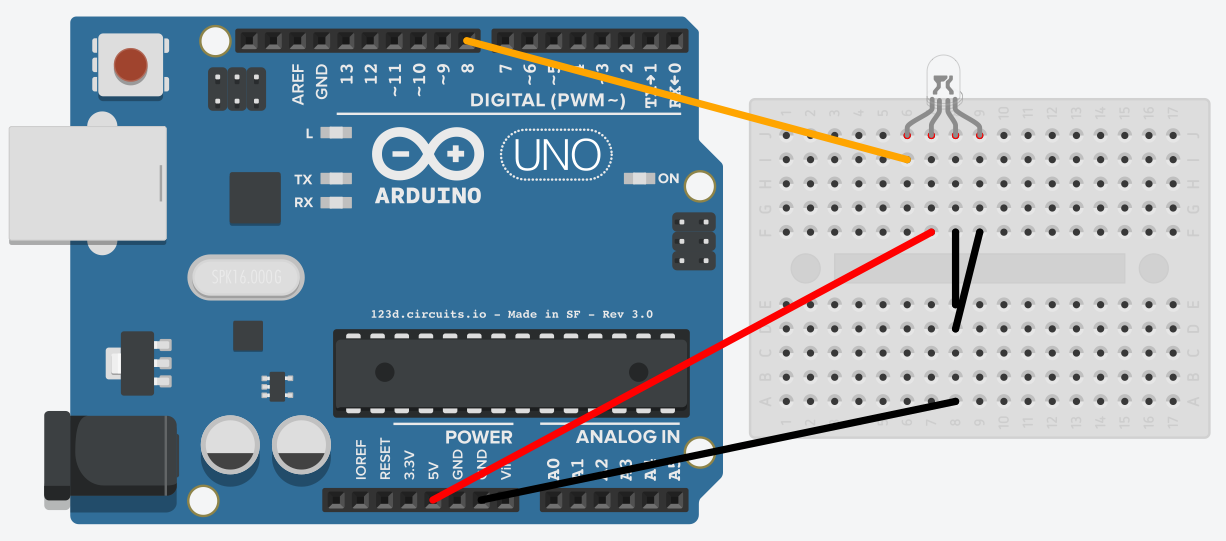
\includegraphics[width=\textwidth]{arduino-pir-wiring.png}
  \caption{The figure depicts wiring for a PIR motion sensor. A LED is shown in
    the figure, for a lack of a PIR component in the software generating the
    wiring schematics.}
  \label{fig:arduino_pir_wiring}
\end{figure}

\subsubsection{Experiments}
\label{sub:Experiments}
In order to determine the reliability of the hardware several experiments are conducted with the PIR sensor.
The tests are all based on data found in the datasheet for the hardware.
The main purpose of the tests is to determine the correlation between real world performance and the hardware specifications
found on the datasheet.
\\\\
Four tests are carried out with one main setup that are applied to all of them. The four consists of the following:

\begin{enumerate}
  \item Sensitivity Test
  \item Angle Test
  \item Distance Test
  \item Delay Time Test
\end{enumerate}
\subsubsection{The Setup}
\label{subs:The Setup}
As aforementioned the setup for all the experiments are identical
that is to ensure consistency of the results by reducing variables, that affects
the results, as much as possible.  The PIR sensor is placed in place surrounded wall
and where other moving objects are limited to a certain degree. In order to ensure that the
results are as precise as possible, all four tests are carried out at the same exact place but
the method of the individual test differs.
The PIR sensor is placed at a certain height and made sure the sensor itself is
sitting still during the tests.
\paragraph{Sensitivity}
\label{par:Sensitivity}

\subparagraph{Hypothesis}
\label{subp:SenHypothesis}
According to the datasheet the PIR sensor will be too sensitive if the distance potentiometer is rotated counter-clockwise.
The sensor should get so sensitivethat the PIR sensor would be triggered by the atmosphere even
if no moving object is existing\cite{datasheet_pir1}.
\subparagraph{Test Procedure}
\label{subp:SenTest Procedure}
The PIR sensor is configured with the distance potentiometer rotated
counter-clockwise as far as possible and the first triggered to test that everything works.
After the sensor is configured every object that can affect the sensor is
removed and the sensor is observed for 30 seconds.
The observation is to determine whether the sensor will detect objects that it is not
supposed to detect and how sensitive the sensor really can is.
\subparagraph{Results}
\label{subp:SenResults}

At the most sensitive setting, nothing was triggered by athmospheric noise. Just
to be sure, the sensor was tested at the least sensitive setting: nothing was
detected, as expected.

\subparagraph{Partial Conclusion}
\label{subp:SenPartial Conclusion}

According to our tests, the atmospheric noise was not detectable at the highest
sensitivity setting.

\paragraph{Angle}
\label{par:Angle}

\subparagraph{Hypothesis}
\label{subp:AngHypothesis}
According to the datasheet of the PIR sensor,
the sensor has a detecting angle of 120 degrees.
The sensor should according to the datasheet not detect any angle above 120 degrees.

\subparagraph{Test Procedure}
\label{subp:AngTest Procedure}
The sensor is placed in a certain position and detecting angle is measured equivalent to
the specified angle found in the datasheet.
For the sake of explanation let the angle above 120 degree be the grey zone and
the detecting area that is within the 120 degree white zone.
A moving object is placed in the grey zone and slowing moving into the white zone.
The PIR sensor should be triggered when the moving object enters the white zone in order
to work exactly as specified in the hardware specifications.
The zone of the moving object and PIR sensor is observed accordingly
and thereby the actual detecting angle is determined.

The test is performed three times on each side at the highest sensitivity of the sensor for consistency.

\subparagraph{Results}
\label{subp:AngResults}

The data results can be seen in \cref{tab:pir_angle}. A plot of this data can be
seen in \cref{fig:pir_angle}.

\begin{figure}[htbp]
\centering
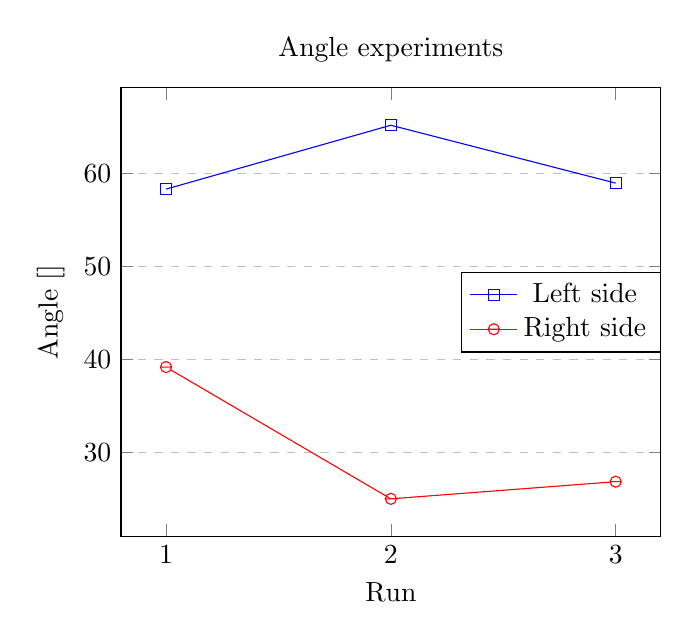
\begin{tikzpicture}
\begin{axis}[
    title={Angle experiments},
    xlabel={Run},
    ylabel={Angle [$\si{\degree}$]},
    xtick={1,2,3},
    legend style={at={(1,0.5)},anchor=east},
    ymajorgrids=true,
    grid style=dashed,
]
\addplot[
    color=blue,
    mark=square,
    ]
    coordinates {
    (1,58.3136)
    (2,65.1905)
    (3,58.9582)
    };
\addlegendentry{Left side}
% asd
\addplot[
    color=red,
    mark=halfcircle,
    ]
    coordinates {
    (1,39.1605)
    (2,24.9812)
    (3,26.8278)
    };
\addlegendentry{Right side}
\end{axis}
\end{tikzpicture}
\caption{Plot of angle experiment}\label{fig:pir_angle}
\end{figure}

\begin{table}[htbp]
\centering
\begin{tabular}{@{}llll@{}}
\toprule
Run & x [cm] & y [cm] & angle [deg] \\ \midrule
1 (left) & 81 & 50 & 58.3136 \\
1 (right) & 79 & 97 & 39.1605  \\ \midrule
2 (left) & 106 & 49 & 65.1905 \\
2 (right) & 82 & 176 & 24.9812 \\ \midrule
3 (left) & 108 & 65 & 58.9582 \\
3 (right) & 88 & 174 & 26.8278 \\ \bottomrule
\end{tabular}
\caption{Results of angle experiments. The x and y columns represent the x and y
  distance from the sensor to the detected person. The angle values are
  calculated by $\arctan (x,y) * \frac{180}{\pi}$}
\label{tab:pir_angle}
\end{table}

\subparagraph{Partial Conclusion}
\label{subp:AngPartial_conclusion}

According to the hypothesis, the sensor should detect motion in an angle of 120
degrees. Our results show that the left side of the sensor is quite correct,
while the other side of the sensor is not very close to 60 $\si{\degree}$.

\paragraph{Distance}

\subparagraph{Hypothesis}

According to the datasheet, the sensor can measure motion from 10 centimeters to
6 meters.

\subparagraph{Test procedure}

The sensitivity setting of the sensor essentially controls the distance. First,
the sensitivity is set to the lowest sensitivity. At that sensitivity, the
sensor should detect motion at a range of 10 centimeters, according to the above
hypothesis.

The sensor is measured by the test conductor approaching the sensor while
waving. Once the sensor detects the motion, the distance from the test conductor
to the sensor is measured. This is done three times to check for consistency. The sensitivity is then upped one unit on the sensor,
and the test conductor measures the distance for the new sensitivity.

\subparagraph{Results}

lowest sensitivity: < 10 centimeters
above + 1: < 10 centimeters
above + 1: 43 cm
above + 1: 123 cm
above + 1: 204 cm
above + 1: 245 cm (acted very strange, long beeps)
above + 1: 275 cm (acted very strange, long beeps)
above + 1: 413 cm
above + 1: 323 cm (acted strange, long beeps)
above + 1: 410 cm
above + 1: 547 cm
above + 1: 600 cm
above + 1: 515 cm

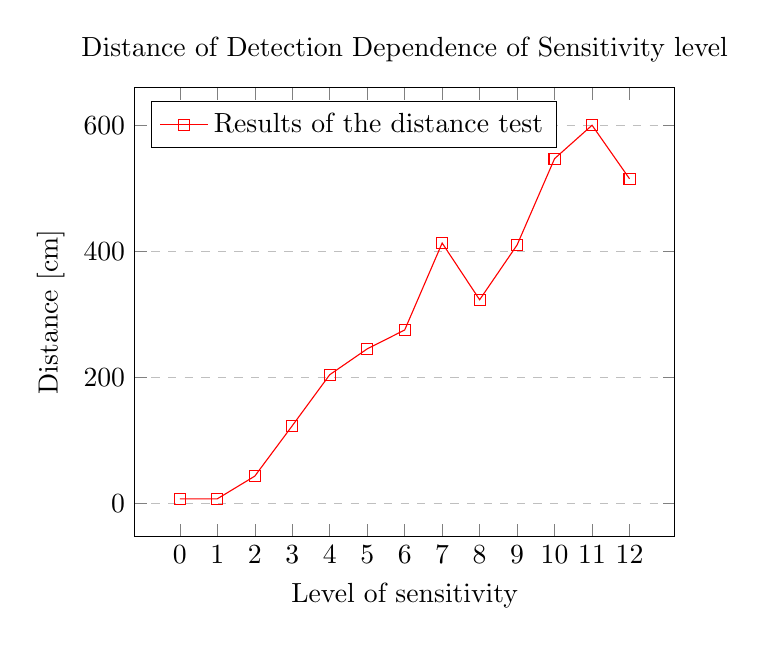
\begin{tikzpicture}
\begin{axis}[
    title={Distance of Detection Dependence of Sensitivity level},
    xlabel={Level of sensitivity},
    ylabel={Distance [cm]},
    %xmin=0, xmax=12,
    %ymin=0, ymax=120,
    xtick={0,1,2,3,4,5,6,7,8,9,10,11,12},
    %ytick={0,20,40,60,80,100,120},
    legend pos=north west,
    ymajorgrids=true,
    grid style=dashed,
]

\addplot[
    color=red,
    mark=square,
    ]
    coordinates {
    (0,7)(1,7)(2,43)(3,123)(4,204)(5,245)(6,275)(7,413)(8,323)(9,410)(10,547)(11,600)(12,515)
    };
    \legend{Results of the distance test}

\end{axis}
\end{tikzpicture}

\subparagraph{Partial conclusion}
The results indicate that there is a correlation between the sensitivity and the detecting distance.
However the sensor behave strange and unpredictable at sensitivity level 7 and 8.
Furthermore the sensor behaved in an unexpected manner  at sensitivity level 3, 4 and 5 by detecting something is was not supposed to detect.
However the maximum distance range seem to be 6meters as stated in the datasheet but at peak sensitivity level
the distance drops down to 5 meter only.

\paragraph{Delay time}

\subparagraph{Hypothesis}

According to the datasheet, the sensor has a delay time of 1 second to 25 seconds.

\subparagraph{Test procedure}

In this experiment, the sensor is set in the non-retriggerable setting (L
position), so the delay time is not extended on additional motion.

First the sensor is adjusted to have the maximum delay time of 25 seconds
according to the above hypothesis. This is then tested by triggering the sensor
and starting a stopwatch simultaneously. When the sensor stops signalling, the
stopwatch is stopped and the actual delay time noted. This is done three times
for each setting of delay time to check for consistency.

The next iteration of the experiment, the delay time potentiometer on the sensor
is rotated one unit, decreasing the value.

\subparagraph{Results}

A plot of the results can be seen in \cref{fig:pir_delay}.

\begin{figure}[htbp]
\centering
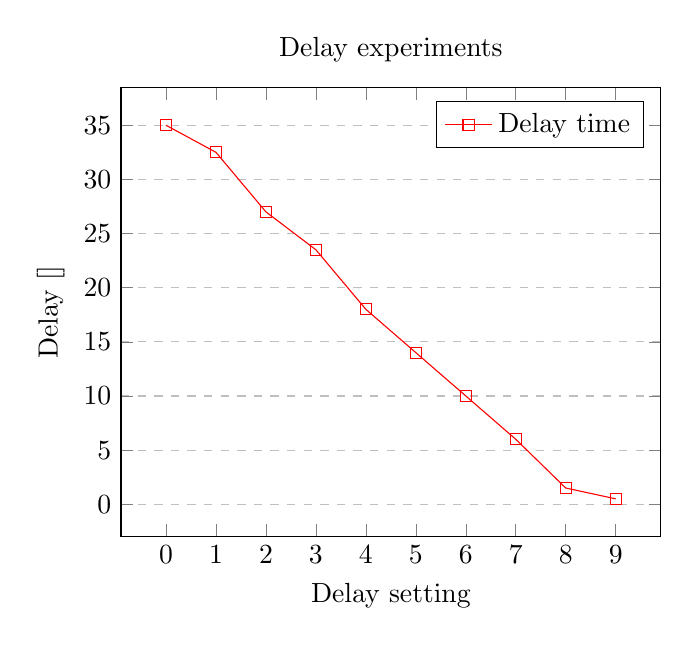
\begin{tikzpicture}
\begin{axis}[
    title={Delay experiments},
    xlabel={Delay setting},
    ylabel={Delay [$\si{\second}$]},
    xtick={0,1,...,9},
    ytick={0,5,...,40},
    legend pos= north east,
    ymajorgrids=true,
    grid style=dashed,
]
\addplot[
    color=red,
    mark=square,
    ]
    coordinates {
    (0,35)
    (1,32.5)
    (2,27)
    (3,23.5)
    (4,18)
    (5,14)
    (6,10)
    (7,6)
    (8,1.5)
    (9,0.5)
    };
\addlegendentry{Delay time}
\end{axis}
\end{tikzpicture}
\caption{Plot of delay experiment. On the x axis number representation of potentiometer, ranging from 0 with highest delay to 9 with lowest. On the y axis the delay time in seconds are shown.}\label{fig:pir_delay}
\end{figure}

\subparagraph{Partial conclusion}

The hypothesis is incorrect. The maximum delay time was recorded to be
around 35 seconds that is a deviation by more than 30\%.
However, the minimum delay time was very close to the value
described in the hypothesis.
